\documentclass[12pt,letterpaper]{article}
\usepackage{fullpage}
\usepackage[top=2cm, bottom=4.5cm, left=2.5cm, right=2.5cm]{geometry}
\usepackage{amsmath,amsthm,amsfonts,amssymb,amscd}
\usepackage{lastpage}
\usepackage{enumerate}
\usepackage[shortlabels]{enumitem}
\usepackage{fancyhdr}
\usepackage{mathrsfs}
\usepackage{xcolor}
\usepackage{graphicx}
\usepackage{listings}
\usepackage{hyperref}

\usepackage[inline]{enumitem}

\setlength{\parindent}{0.0in}
\setlength{\parskip}{0.05in}

\newcommand\course{Complejidad Computacional}
\newcommand\hwnumber{2}                 
\newcommand\NetIDa{Erick Bernal Márquez 317042522} % <-- person #1
\newcommand\NetIDb{José Alejandro Pérez Márquez 310109800}   % <-- person #2
\newcommand\NetIDc{Tania Michelle Rubí Rojas 315121719}  % <-- person #3

\newcommand{\lineaxd}{{\color{brown}\rule{\linewidth}{0.5mm}}}


\pagestyle{fancyplain}
\headheight 35pt
\lhead{\NetIDa}
\lhead{\NetIDa\\\NetIDb\\\NetIDc}                % <-- Comment this line out for problem sets (make sure you are person #1)
\chead{\textbf{\Large Tarea \hwnumber}}
\rhead{\course \\ Semestre 2023-1}
\lfoot{}
\cfoot{}
\rfoot{\small\thepage}
\headsep 1.5em

\begin{document}

\section*{Ejercicio 1}
Sea $M$ una Máquina de Turing cuyo tiempo de ejecución está dado por:

$$f_m(n) = 2n^3(n+3)(n-4)$$

¿Cuáles de las siguientes afirmaciones son verdaderas? Justifica tu repuesta.

\begin{enumerate}[a.]
    \item $f_M \in O(n)$

    \textsc{Solución:} Sean $f(n) = 2n^3(n+3)(n-4)$ y $g(n) = n$. Para que la 
    afirmación fuera cierta necesitaríamos que existieran constantes positivas 
    $c$ y $n_0$ tal que $f(n) \leq cg(n)$, para toda $n \geq n_0$. Así, 
    \begin{align*}
        f(n) \leq cg(n) \\
        2n^3(n+3)(n-4) &\leq cn 
        && \text{definición de $f$ y $g$} \\
        \frac{2n^3(n+3)(n-4)}{n} &\leq \frac{cn}{n} 
        && \text{dividimos entre $n$ en ambos lados} \\ 
        \color{red}2n^2(n+3)(n-4) &\color{red}\leq \color{red} c
        && \text{álgebra}
    \end{align*}

    Pero es claro que no existen constantes $c$ y $n_0$ tal que hagan que la
    desigualdad que está en color rojo sea cierta. Por lo tanto, la afirmación
    es \textbf{falsa}.

    \item $f_M \in O(n^6)$ 

    \textsc{Solución:} Sean $f(n) = 2n^3(n+3)(n-4)$ y $g(n) = n^6$. Esto 
    significa que existen constantes positivas $c$ y $n_0$ tal que 
    $f(n) \leq cg(n)$, para toda $n \geq n_0$. Así, 
    \begin{align*}
        f(n) \leq cg(n) \\
        2n^3(n+3)(n-4) &\leq cn^6
        && \text{definición de $f$ y $g$} \\
        \frac{2n^3(n+3)(n-4)}{n^3} &\leq \frac{cn^6}{n^3} 
        && \text{dividimos entre $n^3$ en ambos lados} \\ 
        2(n+3)(n-4) &\leq cn^3
        && \text{álgebra} \\ 
        2n^2 - 2n -24 &\leq cn^3
        && \text{álgebra}
    \end{align*}

    Sabemos que $n^2 \leq n^3$, por lo que $2n^2 \leq 2n^3$. Además, 
    sabemos que $n \leq n^3$, por lo que $2n \leq 2n^3$. Así, 
    \begin{equation*}
        2n^3 + 2n^3 = 4n^3 \quad \quad \forall n \geq 1
    \end{equation*}

    Por lo tanto, 
    \begin{equation*}
        2n^2 - 2n -24 \leq 4n^3 \quad \quad \forall n \geq 1
    \end{equation*}

    Lo que significa que $c = 4$ y $n_0 = 1$. Por consiguiente, la afirmación
    es \textbf{verdadera}.
    
    \item $f_M \in O(\frac{n^5}{20})$

    \textsc{Solución:} Sean $f(n) = 2n^3(n+3)(n-4)$ y $g(n) = \frac{n^5}{20}$. Esto 
    significa que existen constantes positivas $c$ y $n_0$ tal que 
    $f(n) \leq cg(n)$, para toda $n \geq n_0$. Así, 
    \begin{align*}
        f(n) \leq cg(n) \\
        2n^3(n+3)(n-4) &\leq c \left( \frac{n^5}{20} \right)
        && \text{definición de $f$ y $g$} \\
        2n^3(n+3)(n-4) &\leq \frac{cn^5}{20}
        && \text{multiplicación de fracciones} \\ 
        20(2n^3(n+3)(n-4)) &\leq 20 \left( \frac{cn^5}{20} \right)
        && \text{multiplicamos por $20$ en ambos lados} \\ 
        40n^3(n+3)(n-4) &\leq cn^5
        && \text{álgebra} \\ 
        \frac{40n^3(n+3)(n-4)}{n^3} &\leq \frac{cn^5}{n^3}
        && \text{dividimos entre $n^3$ en ambos lados} \\ 
        40(n+3)(n-4) &\leq cn^2 
        && \text{álgebra} \\ 
        40n^2 - 40n - 480 &\leq cn^2
        && \text{álgebra}
    \end{align*}

    Sabemos que $n \leq n^2$, por lo que $40n \leq 40n^2$ para toda 
    $n \geq 1$. Así, 
    \begin{equation*}
        40n^2 - 40n - 480 \leq 40n^2 \quad \quad \forall n \geq 1
    \end{equation*}

    Lo que significa que $c = 40$ y $n_0 = 1$. Por lo tanto, la afirmación
    es \textbf{verdadera}.
    
    \item $f_M \in \Theta(n^6)$ 

    \textsc{Solución:} Sabemos que para cualesquiera dos funciones $f(n)$ y 
    $g(n)$ tenemos que $f(n) = \Theta(g(n))$ si y sólo si $f(n) = O(g(n))$ y 
    $f(n) = \Omega(g(n))$. Por el inciso $b$ tenemos que $2n^3(n+3)(n-4) = 
    O(n^6)$, así que para determinar si la afirmación es falsa o no, nos falta
    verificar si $2n^3(n+3)(n-4) = \Omega(n^6)$. 

    Sean $f(n) = 2n^3(n+3)(n-4)$ y $g(n) = n^6$. Para que $2n^3(n+3)(n-4) = 
    \Omega(n^6)$ fuera cierto necesitaríamos que existieran constantes positivas 
    $c$ y $n_0$ tal que $cg(n) \leq f(n)$, para toda $n \geq n_0$. Así, 
    \begin{align*}
        cg(n) &\leq f(n) \\ 
        cn^6 &\leq 2n^3(n+3)(n-4) 
        && \text{definición de $f$ y $g$} \\
        \frac{cn^6}{n^3} &\leq \frac{2n^3(n+3)(n-4)}{n^3} 
        && \text{dividimos entre $n^3$ en ambas lados} \\ 
        cn^3 &\leq 2(n+3)(n-4)
        && \text{álgebra} \\ 
        \color{red}cn^3 &\color{red}\leq \color{red}2n^2 - 2n -24
        && \text{álgebra}
    \end{align*}

    Pero sabemos que $n^3 \geq n^2$, por lo que $kn^3 \geq kn^2$ para 
    cualquier $k \geq 1$. Lo que significa que no existen constantes $c$ y 
    $n_0$ tal que hagan que la desigualdad que está en color rojo sea cierta. 
    Por lo tanto, $2n^3(n+3)(n-4) \not = \Omega(n^6)$.

    Por consiguiente, $f_M \not \in \Theta(n^6)$. 
\end{enumerate}
    
\lineaxd

\section*{Ejercicio 2}

Da una descripción general de una máquina de Turing para cada uno de los siguientes lenguajes. Determina la función de complejidad de tiempo en cada caso.

\begin{enumerate}[a.]
    \item $\{ w \in$ $\{$0,1,\#$\}$* $| w$ contiene el triple de 0's que 1's $\}$
    
    \textsc{Solución:}
    \begin{itemize}
        \item Descripción general
        
        Sea $w$ una cadena de entrada para la Máquina $M$.
        \begin{enumerate}[1.]
            \item Si $w$ no contiene ceros ni unos, entonces \textbf{acepta} 
            (por vacuidad se cumple que contiene el triple de ceros que de  
            unos).

            \item Recorremos a $w$ hasta encontrar un cero. Si encontramos un
            \texttt{\char32} (espacio en blanco) antes de encontrar el cero
            entonces \textbf{rechaza} (ya que habremos llegado al final 
                de la cadena). En caso contrario:
                \begin{itemize}[2.1.]
                    \item Reemplazamos el cero por una $X$ y buscamos otro cero 
                    a partir de donde nos quedamos. Si encontramos 
                    \texttt{\char32} antes de encontrar el 
                    cero, entonces \textbf{rechaza} (ya que habremos llegado al 
                    final de la cadena). En caso contrario:
                    \begin{itemize}[2.1.1.]
                        \item Reemplazamos el cero por una $X$ y buscamos otro 
                        cero a partir de donde nos quedamos. Si encontramos 
                        \texttt{\char32} antes de encontrar 
                        el cero, entonces \textbf{rechaza} (hemos llegado al final de la cadena). En caso contrario:
                        \begin{itemize}[2.1.1.1]
                            \item Reemplazamos el cero por una $X$ y regresamos 
                            al inicio de la cadena $w$. 
                        \end{itemize}
                    \end{itemize}
                \end{itemize}

            \item Recorremos $w$ hasta encontrar un uno. Si encontramos un 
            \texttt{\char32} antes de encontrar el uno, 
            entonces \textbf{rechaza}. En caso contrario, reemplazamos el uno 
            por una $Y$ y regresamos al inicio de la cadena $w$. 
            
            \item Repetimos $2$ y $3$ hasta terminar con los ceros de $w$. 

            \item Recorremos a la cadena $w$. Si encontramos un uno, entonces 
            \textbf{rechaza}. En caso contrario, \textbf{acepta}. 
        \end{enumerate}

        Mostraremos un breve ejemplo del algoritmo anterior con una cadena 
        $w = 01000010$. Veamos que $w$ tiene el triple de ceros que de unos. 
        \begin{align*}
            01000010 \\ 
            X1000010 \\ 
            X1X00010 \\ 
            X1XX0010 \\ 
            XYXX0010 \\ 
            XYXXX010 \\ 
            XYXXXX10 \\ 
            XYXXXX1X \\ 
            XYXXXXYX \\ 
            \text{ACEPTA}
        \end{align*}

        \item Complejidad 

        La complejidad de esta máquina es de $O(n^2)$, donde $n$ es la longitud 
        de la cadena de entrada $w$. En el proceso para marcar y buscar un cero 
        o un uno en $w$, en el peor caso, tenemos que recorrer toda la cadena 
        $w$. Así que si $|w| = n$, entonces este proceso nos toma $n$ pasos, 
        lo que implica que nos toma $O(n)$. Esto lo debemos de multiplicar por 
        el número de veces que debemos realizar dicho proceso, esto es, una vez 
        por cada elemento de $w$. Así que como estamos marcando y buscando en 
        tiempo $O(n)$ una cantidad de $n$ veces, entonces tenemos que 
        \begin{equation*}
            O(n) \cdot O(n) = O(n^2)
        \end{equation*}

        es el tiempo total de ejecución. 
    \end{itemize}
    
    \item $\{ w \in$ $\{a,b,c\}$* $| w$ contiene el número de $a$'s en $w >$ número de $b$'s en $w \geq$ número de $c$'s en $w$ $\}$
    
    \textsc{Solución:}
    \begin{itemize}
        \item Descripción general
        
        Sea $w$ una cadena de entrada para la Máquina $M$.
        \begin{enumerate}[1.]
            \item Si $w$ es la cadena vacía, entonces \textbf{acepta} (por vacuidad se cumple que el número de a's es mayor que el número de b's, y que este último número es mayor o igual al número de c's). 
            \item Si $w$ no contiene b's o c's (es una cadena que contiene solamente a's), entonces \textbf{acepta} (ya que el número de 
            a's es mayor al número de b's, que es cero, y particularmente 
            también se cumple que el número de b's es igual al número de c's). 

            \item Recorremos a $w$ hasta encontrar una $b$ y la reemplazamos 
            por una $X$. Regresamos al inicio de $w$, buscamos una $c$ y la 
            reemplazamos por una $Y$. 
            \begin{itemize}
                \item Si después de reemplazar una $b$ por una $X$ ya no 
                encuentro una $c$ en toda la cadena, entonces nos 
                movemos al inicio de $w$. 

                \item Si no encuentro ninguna $b$ para reemplazarla por una 
                $X$, pero sí encuentro una $c$ para reemplazar por una $Y$, 
                entonces \textbf{rechaza}. 

                \item Si ya no encuentro ninguna $b$ para reemplazar ni 
                ninguna $c$ para reemplazar, entonces nos movemos al inicio de 
                $w$.
            \end{itemize} 

            \item Vamos al inicio de la cadena $w$ y repetimos $3$ hasta 
            terminar con todas las b's o todas las c's, pues recordemos que la desigualdad nos permite tener marcar tantas b's como c's y puede que existan b's que no se hayan convertido en $X$.

            \item Recorremos a $w$ hasta encontrar una $a$ y la reemplazamos 
            por una $Z$, regresamos al inicio de $w$, buscamos una $b$ o una 
            $X$ y la reemplazamos por una $W$.
            \begin{itemize}
                \item Si después de reemplazar una $a$ ya no encuentro una $b$ 
                o una $X$ en toda la cadena, entonces \textbf{acepta}. En otro 
                caso, \textbf{rechaza}. 
            \end{itemize} 

            \item Vamos al inicio de la cadena $w$ y repetimos $5$ hasta 
            terminar con todas las a's y todas las b's. 
        \end{enumerate}

        Mostraremos un breve ejemplo del algoritmo anterior con una cadena 
        $w = cbaaba$. Veamos que acepta $w$.  
        \begin{align*}
            cbaaba \\ 
            YXaaba \\ 
            YXaaXa \\ 
            YXZaXa \\ 
            YWZaXa \\ 
            YWZZXa \\ 
            YWZZWa \\ 
            YWZZWZ \\ 
            \text{ACEPTA}
        \end{align*}

        \item Complejidad 
        
        La complejidad de esta máquina de es de $O(n^3)$, donde $n$ es la 
        longitud de la cadena de entrada $w$. En el proceso de reemplazar y 
        buscar una $a, b$ o $c$, en el peor de los casos, dos letras que buscamos están en los extremos de la cadena por lo cual tenemos que recorrer 
        toda la cadena $w$ una cantidad de $n$ veces y luego para el regreso $n-1$, luego $n-2$..., este proceso nos toma $n^2$ pasos, lo que 
        implica que nos toma $O(n^2)$. Esto lo debemos de multiplicar por el 
        número de veces que debemos realizar dicho proceso, esto es, una vez 
        por cada elemento de $w$. Así que como estamos reemplazando y buscando 
        en tiempo $O(n^2)$ una cantidad de $n$ veces, entonces tenemos que 
        \begin{equation*}
            O(n^2) \cdot O(n) = O(n^3)
        \end{equation*} 

        es el tiempo total de ejecución. 
    \end{itemize}
\end{enumerate}

\lineaxd
\section*{Ejercicio 3}
Considera la Máquina de Turing definida por:
 $$M = (\{q_s, q_1, q_2, q_a, q_r\}, \{0.1\}, \{0,1, \_ \}, \delta, q_s, q_a, q_r)$$
 
Describe el lenguaje $L_M$ para cada una de las siguientes definiciones de $\delta$. Para cada inciso:

\begin{itemize}
    \item Justifica tu respuesta agregando un par de ejecuciones (al menos una de aceptación y una de rechazo) para cada inciso.
    
    \item Da la función $f_M(n)$ del tiempo de ejecución de la máquina
\end{itemize}

\begin{enumerate}[a.]
    \item $\delta(q_0, 0) = (q_1, 1, \xrightarrow{}); \delta(q_1, 1) = (q_2, 0, \xleftarrow{})$
    
    $\delta(q_2, 1) = (q_0, 1, \xrightarrow{}); \delta(q_1, \_ ) = (q_a, \_, \xrightarrow{})$
    %%acepta cadenas de la forma 01*, no acepta epsilon
    %%3n -1 analizando k pedo, por cada dos se regresa 1
    
    \item $\delta(q_0, 0) = (q_1, 1, \xrightarrow{}); \delta(q_1, 1) = (q_0, 0, \xrightarrow{})$
    
    $\delta(q_1, \_) = (q_a, \_, \xleftarrow{} )$
    %%acepta de la forma n+1, acepta el 0, no acepta lmabda o epsilon
    
    \item $\delta(q_0, 0) = (q_0, \_, \xrightarrow{}); \delta(q_0, 1) = (q_1, \_, \xrightarrow{})$
    
    $\delta(q_1, 1) = (q_1, \_, \xrightarrow{}); \delta(q_1, \_ ) = (q_a, \_, \xleftarrow{})$
    
\end{enumerate}
* Considera que las reglas (transiciones) que no se indican de manera explícita llevan al estado de rechazo.
\newpage
\begin{enumerate}[a.]
    \item Pondremos de manera gráfica la MT
    \begin{figure}[htb]
        \centering
        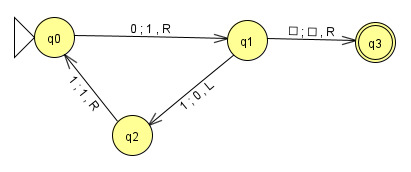
\includegraphics[width=0.5\textwidth]{a.jpg}
    \end{figure}
    

    A primera vista notemos que no acepta la cadena vacia $\epsilon$, acepta el 0 por sí solo y en cuanto leemos más símbolos tenemos que pasar por más estados. Haciendo múltiples ejecuciones nos daremos cuentas que estos estados sirven para verificar que la cadena continue con puros 1's, es decir que no haya 0's después. Concluimos que acepta cadenas de la forma $01^*$
    
    \begin{figure}[htb]
        \centering
        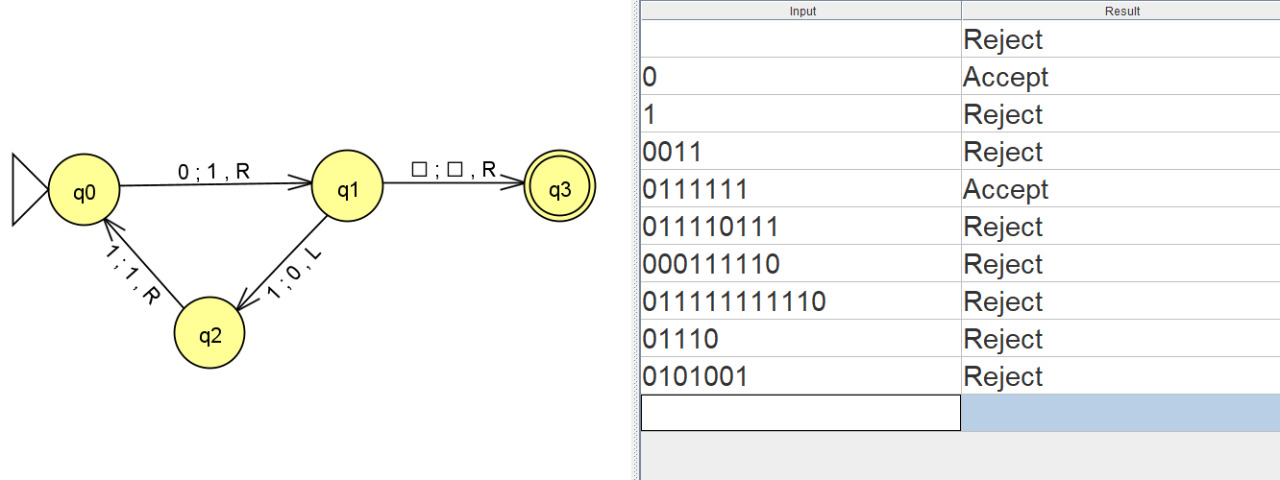
\includegraphics[width=0.70\textwidth]{ares.jpeg}
    \end{figure}
    
    En el peor caso tendremos que recorrer toda la cadena, pero notemos que lo hace de un forma peciluar. Lee el primer simbolo y se regresa, luego lee dos simbolos y se regresa uno, lee dos y se regresa 1, así hasta aceptar la cadena. Siguiendo esta noción si aceptamos una cadena de 1 símbolo la MT hace 2 paso, si aceptamos una cadena de 2 simbolos hacemos 5 pasos, de 3 símbolos 8 pasos, de 4 11 pasos. 
    
    $1 \xrightarrow{}1$ pasos
    
    $2 \xrightarrow{}5$ pasos
    
    $3 \xrightarrow{}8$ pasos
    
    $4 \xrightarrow{}11$ pasos
    
    $5 \xrightarrow{}14$ pasos
    
    $6 \xrightarrow{}17$ pasos
    
    Esta tendencia sigue la ecuación $y = 3n -1$. Así deducimos que la función en tiempo de ejecución de la MT $f_M{(n)}$ es $3n-1$ donde $n$ es el tamaño de la entrada. Además está en el orden de $O(n)$.
    
    \item Pondremos de manera gráfica la MT
    
    \begin{figure}[htb]
        \centering
        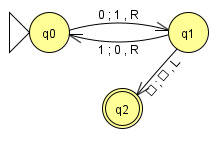
\includegraphics[width=.3\textwidth]{b.jpeg}
    \end{figure}
    
    Notemos que no acepta la cadena vacia, pero sí un 0 sólo, en caso de que el siguiente simbolo sea un 1 el siguiente simbolo necesariamente debe de ser 0 para poder aceptar la cadena, si no es 1 lo rechaza; es decir, acepta las cadenas de la forma $(01)^*0$
    
    \begin{figure}[htb]
        \centering
        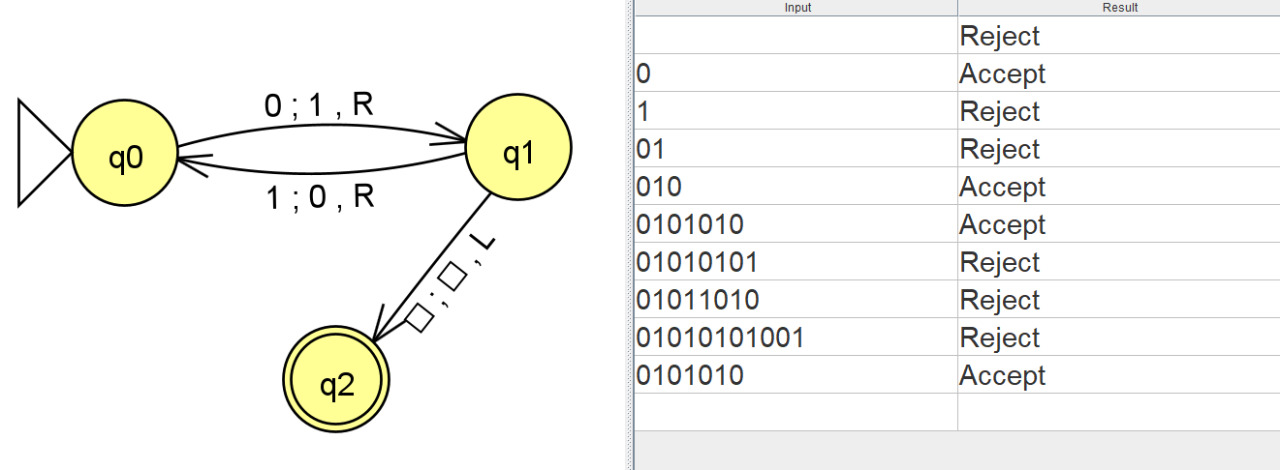
\includegraphics[width=.70\textwidth]{bres.jpeg}
    \end{figure}
    
    Siempre nos movemos a la derecha salvo el último paso para verificar que acabamos de recorrer la cadena, por lo cual $f_M(n)=n+1$ donde $n$ es el tamaño de la entrada, la cual se encuentra en el orden $O(n)$.
    
    \item Pondremos de manera gráfica la MT
    \begin{figure}[htb]
        \centering
        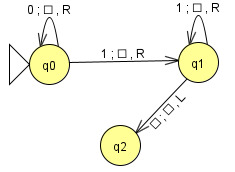
\includegraphics[width=.3\textwidth]{c.jpeg}
    \end{figure}
    \newpage
    De igual manera no acepta la cadena vacia, acepta cualquier cantidad de 0's pues se mantiene en un \textit{ciclo} con el estado $q_0$, luego es necasario aceptar un 1 para avanzar al siguiente estado, de la misma forma se \textit{cicla} en el estado $q_1$ para cualquier cantidad de 1. Por lo cual acepta cadenas de la forma $0^*11^*$
    
    \begin{figure}[htb]
        \centering
        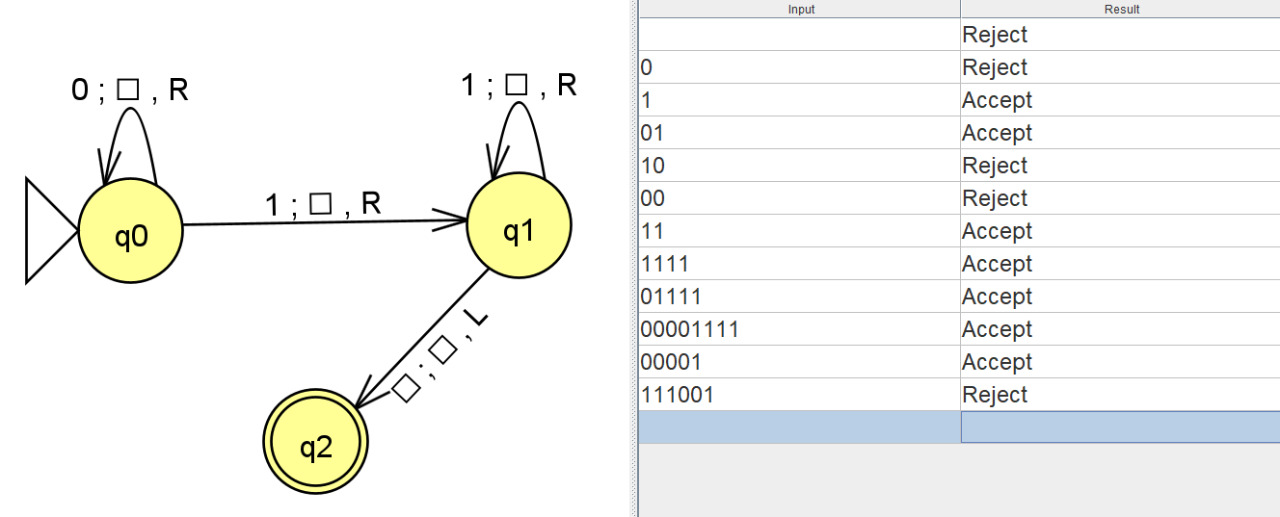
\includegraphics[width=.75\textwidth]{cres.jpeg}
    \end{figure}
    
    De igual manera que el anterior en el peor caso tiene que recorrer toda la cadena, por lo cual 
    $f_M(n)=n+1$ donde $n$ es el tamaño de la entrada. Orden de $O(n)$
\end{enumerate}
    
\lineaxd

\section*{Ejercicio 4}
Sea $L = \{a\#b | a, b$ codifican números enteros positivos en binario y máx(a,b) = $a \}$. Da la descripción completa de una máquina de Turing (incluyendo estados, alfabeto y función de transición) que acepte $L$. Ejemplifica la ejecución de la máquina propuesta mostrando las configuraciones que se producen para las siguientes entradas:

\begin{itemize}
    \item $\lfloor 7 \rfloor \# \lfloor 5 \rfloor \longrightarrow 111 \# 101$
    
    \item $\lfloor 2 \rfloor \# \lfloor 4 \rfloor \longrightarrow 10 \# 100$
    
    \item $\lfloor 1 \rfloor \# \lfloor 1 \rfloor \longrightarrow 1 \# 1$
\end{itemize}
Calcula la complejidad de tiempo, en el peor caso, en función del tamaño de la entrada.

Mostraremos la lógica detrás de la construcción de la Maquina de Turing para hacer más fácil su entendiemiento y analisis.

Primero debemos verificar el tamaño de la entrada, nos interesa que las cadenas a la derecha e izquierda de \# tengan el mismo tamaño o bien el primer número sea mayor que el otro en cuanto a longitud; si el segundo número es mayor entonces ya podemos asegurar que la cadena no pertenece al lenguaje. Esto es lo que hace la primera parte de la MT.

\begin{figure}[htb]
    \centering
    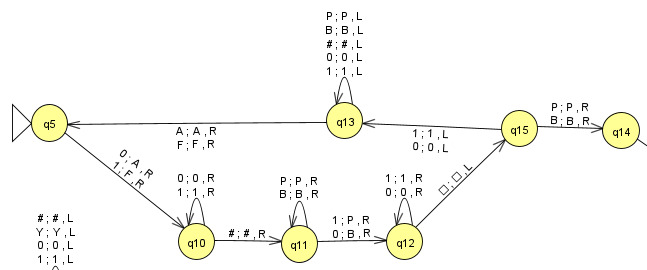
\includegraphics[width=.75\textwidth]{41.jpeg}
\end{figure}

La maquina recorrer toda la cadena y después se regresa, vuelve a recorrerla pero está vez con un símbolo menos, se regresa otra vez y de nuevo la recorre con otro símbolo menos, es decir sigue el clásico patrón $n+(n-1)+(n-2)+(n-3)+...$ (no estamos diciendo que esta sea su $fn$ de complejidad), por lo que su complejidad está en el orden de $O(n^2)$.

Notemos que utilizamos dos 4 símbolos extras: $A,B,P,F$ esto son solamente auxiliares, pues tuvimos que modificar la cadena para llevar el conteo de la longitud, lo que hacen estas letras especiales es ``recordar" el símbolo que tenía la cadena y volverlos a poner.

\begin{figure}[htb]
    \centering
    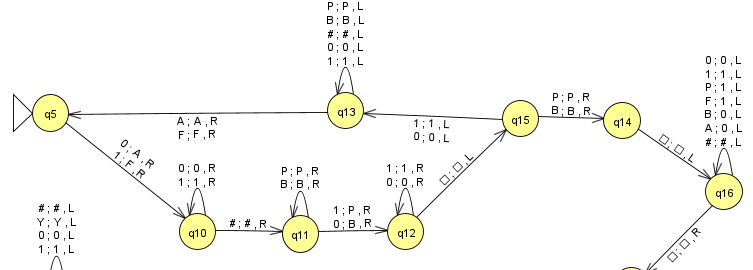
\includegraphics[width=.75\textwidth]{42.jpeg}
\end{figure}

Es de lo que se encarga el estdo $q_{16}$, vemos que lo hace en un estado y siempre a la izquierda hasta llegar al principio de la cadena ya ``recordada". Esto lo hace en un solo recorrido por lo cual tiene complejidad $O(n)$

Una vez que aseguramos ambas cadenas al lado de \# tienen la misma longitud o bien el primer numero es mayor solo queda comparar en sí mismo los números. Esto es lo que hace la segunda parte de la MT.
\newpage

\begin{figure}[htb]
    \centering
    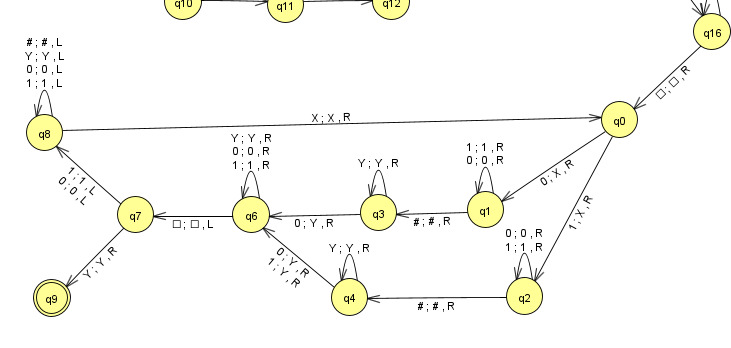
\includegraphics[width=.75\textwidth]{43.jpeg}
\end{figure}

Observemos que de $q_0$ a $q_1$ y $q_2$ hacemos una distinción dependiendo si leemos un 0 o 1, esto es basicamente para hacer la distinción del número mayor.\\
Si leimos primero un 1 y luego, después de pasar el \#, lo comparamos con otro 1 entonces la cadena todavía hay posibilidad de que sea aceptada, lo mismo sí leemos después del \# un 0. Pero si leímos primero un 0 y luego, después de pasar el \#, leemos un 1 entonces en automatico podemos descartar la cadena, pues significa que tenemos un cadena del estilo X01\#Y11 y sabemos que 01 es menor que 11. Esta lógica es basicamente lo que hacen los estados $q_0, q_1, q_2, q_3, q_4, q_6$.

Lo que hace el estado $q_7$ es verificar que el último símbolo de la cadena haya cambiado a Y, así aseguramos que se terminó de leer la cadena.

Al igual que la primera parte de la MT este procedimiento recorre toda la cadena, luego toda la cadena menos un símbolo, luego toda la cadena menos dos simbolos, es decir tiene complejidad $O(n^2)$. La suma de las complejidades es $O(n^2)+O(n)+O(n^2)$ las cuales por propiedades de los ordenes es complejidad $O(n^2)$.

Así definimos la MT en su totalidad como $MT = (Q, \Sigma, \Gamma, \delta, q_5, q_9, q_r)$, donde\\
$Q = \{q_0,q_1,...,q_{16}\}$\\
$\Sigma = \{0,1,\#\}$\\
$\Gamma = \{0,1,\#,\_, A,B,F,P,X,Y\}$\\
$q_5$ es el estado incial\\
$q_9$ es el estado de aceptación\\
$q_r$ son todos los demás estados que no son estados de aceptación.

Las transiciocnes $\delta$ están definidas de manera g´rafica en la MT, ya que una tabla sería más difícil de leer. De igual manera las reglas que no se indican de manera explicita las consideramos como rechazo rechazo.
La Maquina de Turing completa es:
\newpage
\begin{figure}[htb]
    \centering
    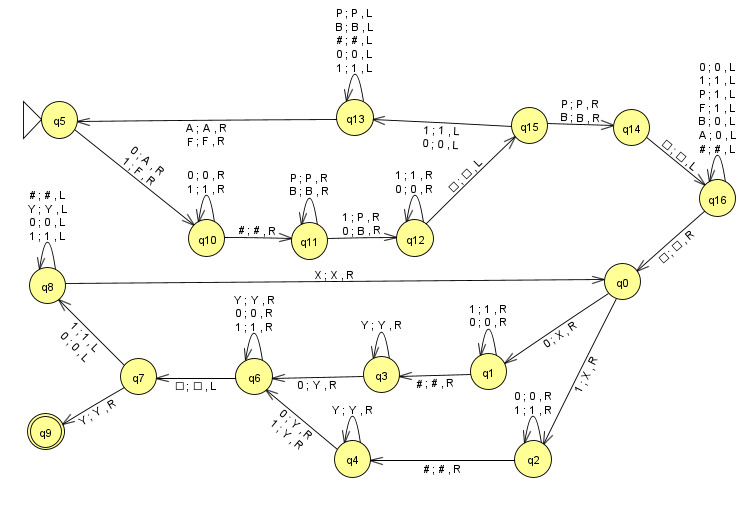
\includegraphics[width=.75\textwidth]{4todo.jpeg}
\end{figure}

Además ponemos algunas entradas.

\begin{figure}[htb]
    \centering
    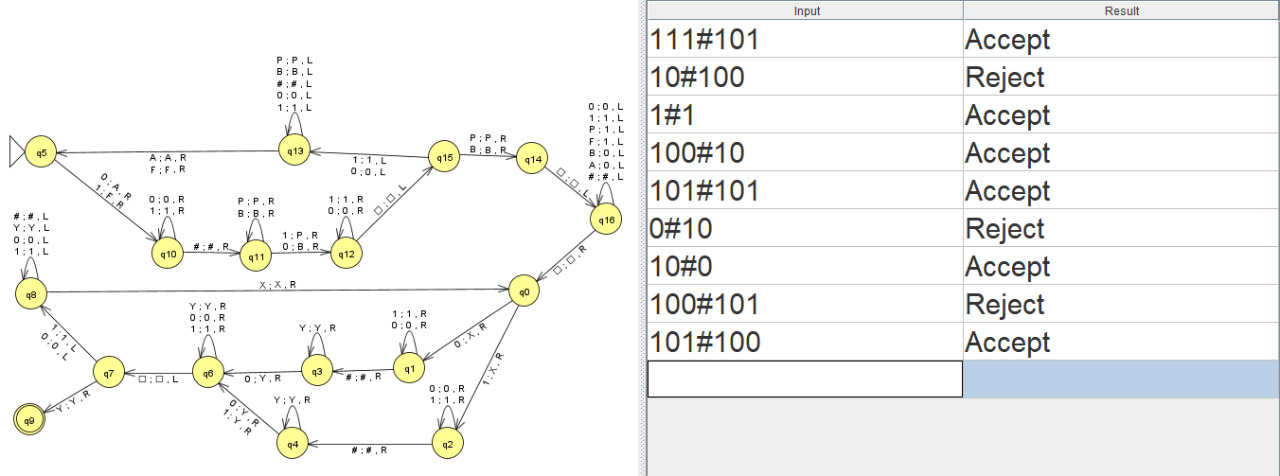
\includegraphics[width=.75\textwidth]{4todores.jpeg}
\end{figure}

Mostraremos las configuraciones de los ejemplos propuestos anteriormente.

\begin{itemize}
    \item $\lfloor 7 \rfloor \# \lfloor 5 \rfloor \longrightarrow 111 \# 101$
    
    $q_5111\#101 \vdash Fq_{10}11\#101 \vdash F1q_{10}1\#101 \vdash F11q_{10}\#101 \vdash F11\#q_{11}101 \vdash F11\#Pq_{12}01 \vdash F11\#P0q_{12}1 \vdash F11\#P01q_{12} \vdash F11\#P0q_{15}1 \vdash F11\#Pq_{13}01 \vdash F11\#q_{13}P01 \vdash F11q_{13}\#P01 \vdash F1q_{13}1\#P01 \vdash Fq_{13}11\#P01 \vdash q_{13}F11\#P01 \vdash Fq_{5}11\#P01 \vdash FFq_{10}1\#P01 \vdash FF1q_{10}\#P01 \vdash FF1\#q_{11}P01 \vdash FF1\#Pq_{11}01 \vdash FF1\#PBq_{12}1 \vdash FF1\#PB1q_{12} \vdash FF1\#PBq_{15}1 \vdash FF1\#Pq_{13}B1 \vdash FF1\#q_{13}PB1 \vdash FF1q_{13}\#PB1 \vdash FFq_{13}1\#PB1 \vdash Fq_{13}F1\#PB1 \vdash FFq_{5}1\#PB1 \vdash FFFq_{10}\#PB1 \vdash FFF\#q_{11}PB1 \vdash FFF\#Pq_{11}B1 \vdash FFF\#PBq_{11}1 \vdash FFF\#PBPq_{12} \vdash FFF\#PBq_{15}P \vdash FFF\#PBPq_{14} \vdash FFF\#PBq_{16}P \vdash^* q_{16}\_111\#101 \vdash q_0111\#101 \vdash Xq_211\#101 \vdash X1q_21\#101 \vdash X1q_21\#101 \vdash X11q_2\#101 \vdash X11\#q_4101 \vdash X11\#Yq_601 \vdash X11\#Y0q_61 \vdash X11\#Y01q_6 \vdash X11\#Y0q_71 \vdash X11\#Yq_801 \vdash X11\#q_8Y01 \vdash X11q_8\#Y01 \vdash X1q_81\#Y01 \vdash Xq_811\#Y01 \vdash q_8X11\#Y01 \vdash Xq_011\#Y01 \vdash XXq_21\#Y01 \vdash XX1q_2\#Y01 \vdash XX1\#q_4Y01 \vdash XX1\#Yq_401 \vdash XX1\#YYq_61 \vdash XX1\#YY1q_6 \vdash XX1\#YYq_71 \vdash XX1\#Yq_8Y1 \vdash XX1\#q_8YY1 \vdash XX1q_8\#YY1 \vdash XXq_81\#YY1 \vdash Xq_8X1\#YY1 \vdash XXq_01\#YY1 \vdash XXXq_2\#YY1 \vdash XXX\#q_4YY1 \vdash XXX\#Yq_4Y1 \vdash XXX\#YYq_41 \vdash XXX\#YYYq_6 \vdash XXX\#YYq_7Y \vdash XXX\#YYYq_9$
    
    Como $q_9$ es estado de aceptación entonces la cadena es aceptada.
    
    \item $\lfloor 2 \rfloor \# \lfloor 4 \rfloor \longrightarrow 10 \# 100$
    
    $q_510\#100 \vdash Fq_{10}0\#100 \vdash F0q_{10}\#100 \vdash F0\#q_{11}100 \vdash F0\#Pq_{12}00 \vdash F0\#P0q_{12}0 \vdash F0\#P00q_{12} \vdash F0\#P0q_{15}0 \vdash F0\#Pq_{13}00 \vdash F0\#q_{13}P00 \vdash F0q_{13}\#P00 \vdash Fq_{13}0\#P00 \vdash q_{13}F0\#P00 \vdash Fq_{5}0\#P00 \vdash FAq_{10}\#P00 \vdash FA\#q_{11}P00 \vdash FA\#Pq_{11}00 \vdash FA\#PBq_{12}0 \vdash FA\#PB0q_{12} \vdash FA\#PBq_{15}0 \vdash FA\#Pq_{13}B0 \vdash FA\#q_{13}PB0 \vdash FAq_{13}\#PB0 \vdash Fq_{13}A\#PB0 \vdash FAq_5\#PB0$
    
    No hay transiciones definidas a en es estado con tal símbolo de entrada, por lo cual consideramos como rechazo
    
    \item $\lfloor 1 \rfloor \# \lfloor 1 \rfloor \longrightarrow 1 \# 1$
    
    $q_51\#1 \vdash Fq_{10}\#1 \vdash F\#q_{11}1 \vdash F\#Pq_{12} \vdash F\#q_{15}P \vdash F\#Pq_{14} \vdash F\#q_{16}P \vdash Fq_{16}\#1 \vdash q_{16}F\#1 \vdash q_{16}\_1\#1 \vdash  q_{0}1\#1 \vdash Xq_2\#1 \vdash X\#q_41 \vdash X\#q_4Y \vdash X\#q_7Y \vdash X\#Yq_9$
    
    Como $q_9$ es estado de aceptación entonces la cadena es aceptada
\end{itemize}

\lineaxd

\section*{Ejercicio 5}

\textbf{Investiga en qué son las funciones de tiempo “construibles” (Time-constructible functions)}

Dada  $T: \mathbb{N} \rightarrow \mathbb{N}$  decimos que:

\begin{enumerate}
    \item T es de tiempo construible si existe $n_0$ una constante y una máquina de Turing M que computa a la función 
    $$ 1^{n} \rightarrow  T(n)  $$ en tiempo $T(n)$ para toda $n \geq n_0$
\end{enumerate}

\newpage

También podemos considerar la siguiente definición

Dada  $T: \mathbb{N} \rightarrow \mathbb{N}$  decimos que:

\begin{enumerate}[2.]
  \item T es de tiempo construible si existe $n_0$ una constante y una máquina de Turing M que computa a la función 
    $$ 1^{n} \rightarrow \lfloor T(n) \rfloor $$ en tiempo $O(T(n))$ para toda $n \geq n_0$ (donde $\rightarrow \lfloor T(n) \rfloor $ es la representación binaria de $T(n)$. De hecho también podemos considerar $ 1^{n} \rightarrow 1^{T(n)} $ en lugar de $ 1^{n} \rightarrow \lfloor T(n) \rfloor$)
\end{enumerate}

\textbf{Elige dos de las siguientes funciones y demuestra que son de tiempo construibles:}

\begin{enumerate}[a.]
    \item $2n log(n)$ 
    \item $3n^2$
    \item $3^n$
\end{enumerate}

Elegimos demostrar $3^{n}$ y $2n log(n)$

    \begin{enumerate}[a.]
       
        \item $3^n$ : Queremos construir una Máquina de Turing que acepte : \\
        
        $\{111, 111111111, 111111111111111111111111111, ..., 1^{f(n)}\}  $ \\
        
        es decir $1^{f(n)}$ para toda $n\in \mathbb{N}$ donde $f(n)=3^n$ \\

Usamos una máquina de dos cintas. En la primera cinta vamos a copiar la entrada $1^{n}$ para comparar. La idea es generar las cadenas posibles una por una en la cinta 2 y luego compararlas, hasta que la cinta 2 sea más larga que la cinta 1.\\

La cinta 2 crecería de $3^n$ a $3^{n+1}$ entre cada comparación. Se puede hacer esto triplicando cada $1$ de la cadena anterior. Hacemos esto agregando una $x$ como marcador al final de la cadena anterior y luego borro los 1's a la izquierda, y para cada uno agrego tres 1's a la derecha.\\

Intuitivamente quedaría así: 

1 (y luego comparamos la cinta 1 y dos) \\ 
-1x\\
—x111\\
—-111  (y luego comparamos la cinta 1 y dos) \\ 
—-111x\\
——11x111\\
——-1x111111\\
——- x111111111\\
——— 111111111  (y luego comparamos la cinta 1 y dos) \\
——— 111111111x\\
———- 11111111x111\\
etc ..        \\

 \item $2n log(n)$ : Dado que $2n$ y $log(n)$ son funciones tiempo-construibles su producto también. La demostración de que $2n$ es tiempo-construible es análoga a la de $3^{n}$ pero  cambiando el hecho de que la máquina de Turing debe aceptar. 

        $\{11, 1111, 111111, ..., 1^{2n}\}  $ \\

Parecido para $log(n)$ que se construye en tiempo $O(log(n))$\\

Intutivamente otra forma de hacerlo es primero representar a 2n  en binario; luego el producto de 2n y log(n); el último está acotado por $O(2n log(n))$ pasos.
    
    \end{enumerate}

\textbf{Da otros ejemplos (diferentes a los del inciso anterior) de funciones de tiempo construible.}

SOLUCIÓN: (De hecho cualquier función polinomial, exponencial o factorial es una función tiempo construible).

\begin{enumerate}[a.]
        \item $n^2$
    
        \item $2^n$
    \end{enumerate}
    
\textbf{Da un par de ejemplos de funciones que no son de tiempo construible. Justifica por qué no lo son.}

SOLUCIÓN:
\begin{enumerate}[a.]
        \item Evidentemente alquier función que no sea computable no es tiempo construible. 

        \item $\lfloor log (x+1) \rfloor$ no es tiempo construible pues  para determinar apenas el tamaño de x le toma a la máquina hacerlo en $|x|$ pasos.
        
        \item Por el Time Hierarchy Theorem\footnote{Time Hierarchy Theorem : Si g y f son funciones tiempo construibles que satisfacen que $f(g) log f(n) = o (g(n)) $ entonces $DTIME (f(n)) \subsetneq DTIME (g(n))$ donde $DTIME(T(n))$ es el conjunto de todas las funciones booleanas (que de hecho se codifican en el lenguaje $L_f = {x : f(x) = 1}.$) que son computables en tiempo $c T(n)$ para alguna constance c.} sabemos que $DTIME (n) \subsetneq DTIME (n^{2})$ por lo que si tomamos una función $f$ que esté en $DTIME (n^{2}) - DTIME (n)$ y la máquina de Turing $M$ correspondiente al lenguaje $L_f$, se tiene que $M$ decide si una cadena está en el lenguaje $L_f$ en tiempo $O(n^{2})$ y $\omega(n)$. Así, si definimos la función $h(n)=2n + M(n)$ esta función no es tiempo construible (pues está definida en función de M).
        
\end{enumerate}




    
\section*{Ejercicio 6}

En los programas de las máquinas de Turing hay operaciones qué son frecuentes de utilizar como pasos intermedios, una de estas operaciones es llamada “desplazamiento”.

Un desplazamiento consiste en mover todo el contenido de la cinta una posición a la derecha o la izquierda, a partir de una posición específica, y luego regresar la cabeza de la máquina
a dicha posición.

\begin{enumerate}[a.]
    \item Indica con todo detalle cómo realizar esta operación:

Resolveremos el ejercicio para cuando se trata de desplazar el contenido de la cinta a la izquierda.

Descripción:

1. Sea w una entrada (cadena) de tamaño n (digamos $x_1x_2x_3...x_n$ para la máquina M y sea $m<n$ el índice de la posición a partir de la cual queremos desplazar a la izquierda toda la cadena)\\
2. Nos posicionamos hasta el principio de la cadena (es decir nos movemos m-1 posiciones a la izquierda), leemos $x_1$ y copiamos $x_1$ \\
3. Nos movemos a la izquierda una posición y reemplazamos su contenido por la letra $x_1$\\
4. Nos movemos a la derecha dos posiciones, leemos y copiamos la letra $x_2$ \\
5. Nos movemos a la izquierda tres posiciones y reemplazamos su contenido por la letra $x_2$\\
6. Nos movemos a la derecha cuatro posiciones, leemos y copiamos la letra $x_3$ \\
7. Nos movemos a la izquierda cinco posiciones y reemplazamos su contenido por la letra $x_3$\\
.\\
.\\
.\\
n-1. Nos movemos a la derecha n-1 posiciones, leemos y copiamos la letra $x_{n-1}$\\ 
n.  Nos movemos a la izquierda n posiciones y reemplazamos su contenido por la letra $x_{n-1}$\\
n+1. Nos movemos a la derecha n+1 posiciones, leemos y copiamos la letra $x_{n}$\\ 
n+2.  Nos movemos a la izquierda n+2 posiciones y reemplazamos su contenido por la letra $x_{n}$ y de hecho ya nos encontramos en la cabeza de la máquina\\
    
    \item Considera la siguiente configuración: $110q101$ donde $q$ es el estado inicial para ejecutar la operación de desplazamiento. De acuerdo a la descripción del inciso anterior, muestra todas las configuraciones hasta completar la operación.\\

La configuración $110q101$ nos dice que $w=110q101$ por lo que $n=7$ y $m=4$. Suponemos que $q=0$\\

Empezamos por mover a $q$ tres posiciones a la izquierda, leemos(en este caso leemos $x_1=1$), nos movemos a la izquierda una posición y escribimos lo que leímos es decir 1.\\

Nos movemos ahora dos posiciones a la derecha, leemos (en este caso $x_2=1$), nos movemos a la izquierda tres posiciones y escribimos lo que leímos es decir 1. \\

Nos movemos ahora cuatro posiciones a la derecha, leemos (en este caso $x_3=0$), nos movemos a la izquierda cinco posiciones y escribimos lo que leímos es decir 0. \\

Nos movemos ahora seis posiciones a la derecha, leemos (en este caso $x_4=0$), nos movemos a la izquierda siete posiciones y escribimos lo que leímos es decir 0. \\

Nos movemos ahora ocho posiciones a la derecha, leemos (en este caso $x_5=1$), nos movemos a la izquierda nueve posiciones y escribimos lo que leímos es decir 1. \\

Nos movemos ahora diez posiciones a la derecha, leemos (en este caso $x_6=0$), nos movemos a la izquierda once posiciones y escribimos lo que leímos es decir 0. \\

Nos movemos ahora doce posiciones a la derecha, leemos (en este caso $x_7=1$), nos movemos a la izquierda trece posiciones y escribimos lo que leímos es decir 1. \\
    
    \item ¿Cuál es la complejidad de esta operación?

El número de pasos es la suma de los primeros 13 números: ($\frac{13(13+1)}{2}$)  más los tres pasos que recorrimos al principio, por lo que su complejidad está en el orden de $O(n(n^2))$.
    
    \item Explica o justifica por qué esta operación puede ser útil.

La operación puede ser útil pues en muchos casos es más óptimo tener un contenido en determinada posición.
    
\end{enumerate}

\lineaxd

\section*{Referencias}
Notación asintótica: \url{https://cs.famaf.unc.edu.ar/~hoffmann/md18/04.html}

Software utilizado para la creación y ejecución de las MT: \url{https://www.jflap.org/}

Definición de Tiempo Construible, página 117:
\url{https://www.math.univ-toulouse.fr/~msablik/Cours/Complexite/Slide-Complexite.pdf}


\end{document}
